

\minitoc

In this chapter we come to the core of this thesis, namely to test how the Fribourg construction performs on real test automata. We are interested in two things. First, how the different versions of the Fribourg construction compare to each other. That is, with which optimisations the Fribourg construction is most efficient. Second, we compare the Fribourg construction to other complementation constructions. We can refer ot the first type of investigations as the \textit{internal} tests, and to the second one as the \textit{external} tests.

To do these investigations, we implemented the Fribourg construction as a plugin for an \om-automata manipulation tool called GOAL. GOAL already contains implementations of the most important Büchi complementation constructions. That is, with our plugin, the Fribourg construction lives next to these other constructions in the GOAL tool, and can be easily compared to them. With the plugin in place, we then performed the actual internal and external tests. To do so, we defined a set of test data consisting of totally 22.000 automata. The performance investigation consists then in basically complementing each of these automata with the different constructions, and comparing the results. Our main performance metric is the number of generated states for the output automata. The computations, which due to the complexity of Büchi complementation are quite heavy, were executed on a high-performance computing cluster at the University of Bern, Switzerland.

In this chapter, we are going to describe each of these points, including our concrete experiment setup. The results of the tests are presented and discussed in Section~\ref{results}.


\section{GOAL}
\label{goal}
GOAL stands for Graphical Tool for Omega-Automata and Logics and has been developed at the National University of Taiwan since 2007~\cite{2007_goal,2008_goal_ext}. The tool is based on the three pillars, \om-automata, temporal logic formulas, and games. It allows to create instances of each of these types, and manipulate them in a multitude of ways. Relevant for our purposes are the \om-automata capabilities of GOAL.

With GOAL, one can create Büchi, Muller, Rabin, Streett, parity, generalised Büchi, and co-Büchi automata, either by manually defining them, or by having them randomly generated. It is then possible to perform a plethora of operations on these automata. The entirety of provided operations are too many to list, but they include containment testing, equivalence testing, minimisation, determinisation, conversions to other \om-automata types, product, intersection, and, of course, complementation.

All this is accessible by both, a graphical and a command line interface. The graphical interface is shown in Figure~\ref{goal_gui}. Automata are displayed in the main editor window of the GUI. They can be freely edited, such as adding or removing states and transitions, and arranging the layout. There are also various layout algorithms for automatically laying out large automata. Most of the functionality provided by the graphical interface is also accessible via a command line mode. This makes it suitable for automating the execution of operations.

\begin{figure}
\begin{center}
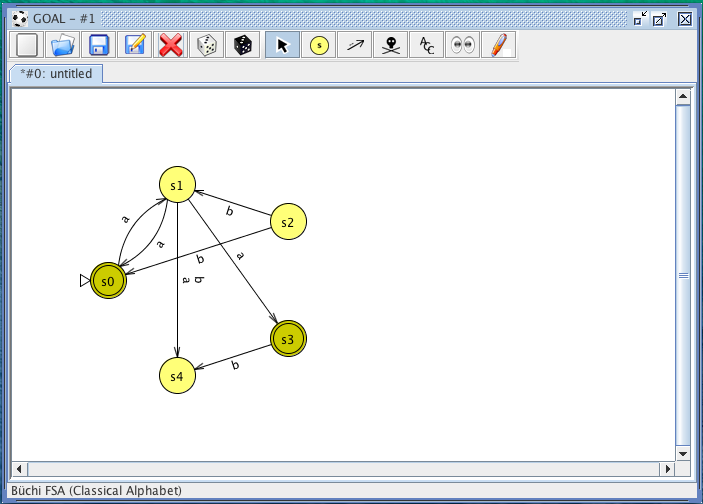
\includegraphics[scale=0.5]{figures/goal_gui.png}
\caption{Graphical interface of GOAL.}
\label{goal_gui}
\end{center}
\end{figure} 

For storing automata, GOAL defines an own XML-based file format, called GOAL File Format, usually indicated by the file extension gff.

An important design concept of GOAL is modularity. GOAL uses the Java Plugin Framework (JPF)~\footnote{http://jpf.sourceforge.net/}, a library for building modular and extensible Java applications. A JPF application defines so-called extension points for which extensions are provided. These extensions contain the actual functionality of the application. Extensions and extension points are bundled in plugins, the main building block of a JPF application. It is therefore possible to extend an existing JPF application by bundling a couple of new extensions for existing extensions points in a new plugin, and installing this plugin into the existing application. On the next start of the application, the new functionality will be included, all without requiring to recompile the existing application or to even have its source code.

GOAL provides a couple of extensions points, such as \textit{Codec}, \textit{Layout}, or \textit{Complementation Construction}. An extension for \textit{Codec}, for example, allows to add the handling of a new file format which GOAL can read from and write to. With an extension for \textit{Layout} one can add a new layout algorithm for laying out automata in the graphical interface. And an extension to \textsf{Complementation Construction} allows to add a new complementation construction to GOAL. This is how we added the Fribourg construction to GOAL, as we will further explain in Section~\ref{implementation}.

There are a couple of Büchi complementation constructions pre-implemented in GOAL. Table~\ref{goal_constructions} summarises them, showing for each one its name on the graphical interface and in the command line mode, and the reference to the paper introducing it. As can be seen, the most important representants of all the four approaches (Ramsey-based, determinisation-based, rank-based, and slice-based, see Chapter~\ref{background}) are present. In addition to the listed constructions, GOAL also contains Kurshan's construction and classic complementation. These are for complementing DBW and NFA/DFA, respectively, and thus not relevant to us.

\begin{table}
\caption{The complementation constructions implemented in GOAL (version 2014-11-17).}
\begin{center}
\begin{tabular}{|l|l|l|}
\hline
Name & Command line & Reference \\
\hline
Ramsey-based construction & ramsey & Sistla, Vardi, Wolper (1987)~\cite{PrasadSistla1987217} \\
\hline
Safra's construction & safra & Safra (1988)~\cite{1988_safra_1} \\
\hline
Modified Safra's construction & modfiedsafra & Althoff (2006)~\cite{2006_althoff} \\
\hline
Muller-Schupp construction & ms & Muller, Schupp (1995)~\cite{Muller199569} \\
\hline
Safra-Piterman construction & piterman & Piterman (2007)~\cite{2007_piterman} \\
\hline
Via weak alternating parity automaton & wapa & Thomas (1999)~\cite{1999_thomas} \\
\hline
Via weak alternating automaton & waa & Kupferman, Vardi (2001) \cite{Kupferman:2001} \\
\hline
Rank-based construction & rank & Schewe (2009) \cite{schewe2009buchi} \\
\hline
Slice-based construction (preliminary) & slice -p & Vardi, Wilke (2007) \cite{vardi2007automata} \\
\hline
Slice-based construction & slice & Kähler, Wilke (2008) \cite{2008_kaehler} \\
\hline
\end{tabular}
\end{center}
\label{goal_constructions}
\end{table}

One of the constructions can be set as the default complementation construction. It is then possible to invoke this construction with the shortcut Ctrl-Alt-C. Furthermore, the default complementation constructions will be used for the containment and equivalence operations on Büchi automata, as they include complementation.

Complementation constructions in GOAL can define a set of options that can be set by the user. In the graphical interface this is done at the start of the operations via a dialog window, in the command line mode the options are specified as command line arguments. Figure~\ref{goal_complementation_options} shows the options dialog of the Safra-Piterman construction. Complementation options allow to play with different configurations and variants of a construction, and we will make use of them for including the optimisations presented in Chapter~\ref{fribourg_construction} to our implementation of the Fribourg construction.


\begin{figure}
\begin{center}
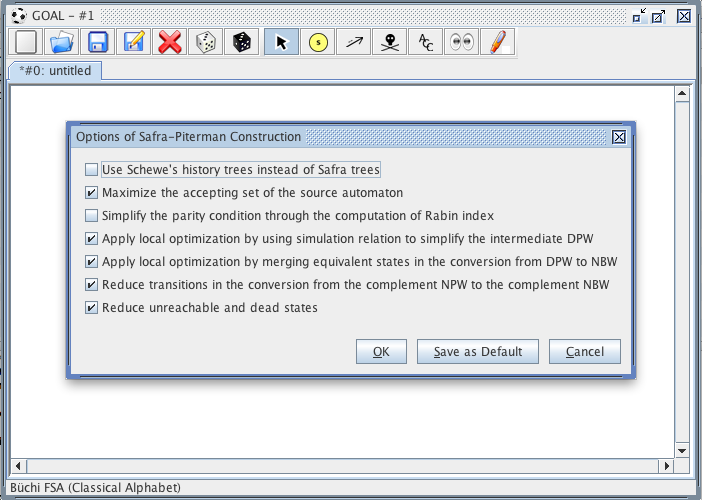
\includegraphics[scale=0.5]{figures/goal_complementation_options.png}
\caption{Complementation constructions in GOAL can have a set user-selectable options. Here the options of the Safra-Piterman construction.}
\label{goal_complementation_options}
\end{center}
\end{figure}

For most complementation constructions (all listed in Table~\ref{goal_constructions} except the Ramsey-based construction) there is also a version for step-by-step execution. In this case, the constructions define so-called steps and stages, through which the user can iterate independently. This is a great way for understanding how a complementation construction works, and for investigating specific cases in order to potentially further improve the construction. 


\section{Implementation of the Fribourg Construction as a GOAL Plugin}
\label{implementation}
We implemented the Fribourg construction, including its optimisations, in Java as a plugin for GOAL. This means that after installing out plugin to an existing GOAL installation\footnote{As the plugin interfaces of GOAL have recently changed, the can be used only for GOAL versions 2014-11-17 and newer.}, the Fribourg construction will be an integral part of GOAL and can be used in the same way as any other pre-existing complementation construction.

\subsection{Options for the Fribourg Construction}
To keep the Fribourg construction flexible, we made use of options. The three optimisations described in Section~\ref{optimisations} are presented to the user as selectable options. Additionally, we included several further options. Table~\ref{goal_fribourg_options} lists them all. For convenience, we use for each options a short code name, which is also used as the option name in the command line mode.

\begin{table}
\caption{The options for the Fribourg construction.}
\begin{center}
\begin{tabular}{|l|l|}
\hline
Code & Description \\ \hline
m1 & Component merging optimisation \\ \hline
m2 & Single 2-coloured component optimisation \\ \hline
r2c & Deleting states with rightmost colour 2, if automaton is complete \\ \hline
c & Make input automaton complete \\ \hline
macc & Maximise accepting states of input automaton \\ \hline
r & Remove unreachable and dead states from output automaton \\ \hline
rr & Remove unreachable and dead states from input automaton \\ \hline
b & Use the ``bracket notation'' for state labels \\ \hline
\end{tabular}
\end{center}
\label{goal_fribourg_options}
\end{table}

The first three items in Table~\ref{goal_fribourg_options}, m1, m2, and r2c, correspond to the optimisations M1, M2, and R2C, described in Section~\ref{optimisations}. As the M2 optimisation requires M1, our implementation makes sure that the m2 option can only be selected if also the m1 option is selected. The \tec{c} option, for making the input automaton complete before starting the actual construction, is intended to be used with the \tec{r2c} option. In this way, the R2C optimisation can be forced to apply. This idea results from previous work that investigated whether making the input automaton complete plus the application of the R2C optimisation brings an improvement over the bare Fribourg constructoin~\cite{2013_bsc_goettel}. The result was negative, that is, the construction performs worse with this variant on practical cases. Also note that using the \tec{c} option alone, very likely decreases the performance of the construction, because the automaton is made bigger if it is not complete.

The \tec{macc} and \tec{r} options are common among the other complementation constructions in GOAL. The first one, \tec{macc}, maximises the accepting set of the input automaton. That means, it makes as many states accepting as possible without changing the automaton's language. This should help to make the complement automaton smaller. The \tec{r} options prunes unreachable and dead states from the complement automaton. Unreachable states are states that cannot be reached from the initial states, and dead states are states from where no accepting state can be reached. Clearly, all the runs containing an unreachable or dead state are not accepting, and thus these states can be removed from the automaton without changing its language. The complement automaton can in this way be made smaller. The \tec{rr} option in turn removes the unreachable and dead states from the \emph{input} automaton. That is, it makes the input automaton smaller, before the actual construction starts, what theoretically results in smaller complement automaton.

Finally, the \tec{b} option affects just the display of the state labels of the complement automaton. It uses an alternative notation which uses different kinds of brackets, instead of the explicit colour number, to indicate the colours of sets. In particular, 2-coloured sets are indicated by square brackets, 1-coloured sets by round parenthesis, and 0-coloured sets by curly braces. Sets of states of the upper part of the automaton are enclosed by circumflexes. This notation, although being very informal, has proven to be very convenient during the development of the construction.

When we developed the plugin, we aimed for a complete as possible integration with GOAL. We integrated the Friboug construction in the graphical, as well as in the command line interface. We added a step-by-step execution of the construction in the graphical interface. We provided that customised option configurations can be persistently saved, and reset to the defaults at any time. We also integrated the Fribourg construction in the GOAL preferences menu so that it can be selected as the default complementation construction. In this way, it can be invoked with a key-shortcut and it will also be used for the containment and equivalence operations. Our goal is that once the plugin is installed, the Fribourg construction is as seamlessly integrated in GOAL as all the other pre-existing complementation construction.

The complete integration allows us to publish the plugin so that it can be used by other GOAL users. At the time of this writing, the plugin is accessible at \url{http://goal.s3.amazonaws.com/Fribourg.tar.gz} and also over the GOAL website\footnote{http://goal.im.ntu.edu.tw/}. The installation is done by simply extracting the archive file and copying the contained folder to the \tec{plugins/} folder in the GOAL system tree. No compilation is necessary. The same plugin and the same installation procedure works FOR Linux, Mac OS X, Microsoft Windows, and other operating systems that run GOAL.

Since between the 2014-08-08 and 2014-11-17 releases of GOAL certain parts of the plugin interfaces have changed, and we adapted our plugin accordingly, the currently maintained version of the plugin works only with GOAL versions 2014-11-17 or newer. It is thus essential for any GOAL user to update to this version in order to use our plugin.

\section{Verification of the Implementation}
Of course it is needed to test whether our implementation produces correct results. That is, are the output automata really the complements of the input automata? We chose doing so with an empirical approach, taking one of the pre-existing complementation constructions in GOAL as the ``ground truth''. We can then perform what we call complementation-equivalence tests. We take a random Büchi automaton and complement it with the ground-truth construction. We then complement the same automaton with our implementation of the Fribourg construction, and check whether the two complement automata are equivalent. Provided that the ground-truth construction is correct, we can show in this way that our construction is correct for this specific case.

We performed complementation-equivalence tests for the Fribourg construction with different option combinations. In particular, we tested the configurations \tec{m1}, \tec{m1}+\tec{m2}, \tec{c}+\tec{r2c}, \tec{macc}, \tec{r}, \tec{rr}, and the construction without any options. For each configuration we tested 1000 random automata of size 4 and with an alphabet of size 2 to 4. As the ground-truth construction we chose the Safra-Piterman construction. In all cases the complement of the Fribourg construction was equivalent to the complement of the Safra-Piterman construction.

Doubtlessly, it would be desirable to test more, and especially bigger and more diverse automata. However, by doing so one would quickly face practical problems due to long complementation times with bigger automata and larger alphabets, and high memory usage. For our current purpose, however, the tests we did are enough for us to be confident that our implementation is correct.

\section{Test Data}
For our set of sample automata, we chose to adopt the test set that has been created and used for another empirical performance comparison of Büchi complementation constructions by Tsai et al.~\cite{2010_tsai} (the first author, Tsai, being the main author of GOAL). This test set consists of 11000 automata of size 15, and 11000 automata of size 20. Each set of 11000 automata consists of 110 groups containing 100 automata each. The 110 groups result from the cartesian product of 11 transitions densities and 10 acceptance densities.

At this point, we have to explain the notions of transition and acceptance densitiy, as they are defined in~\cite{2010_tsai} and also implemented in GOAL. The transition density defines the number of transitions in an automaton. In particular, if the transition density is $t$ and the automaton has $n$ states, then the automaton contains $tn$ transitions for every symbol of the alphabet. In other words, the transition density is the average number of outgoing (and incoming) transitions of a state for each symbol of the alphabet. The transition densities in the test set range from 1 to 3 in steps of 0.2, that is, there are the 11 instances 1.0, 1.2, 1.4, 1.6, 1.8, 2.0, 2.2, 2.4, 2.6, 2.8, 3.0. The acceptance density in turn is the percentage of states that are accepting states. It is thus a number between 0 and 1. In the test set, the 10 acceptance density classes range from 0.1 to 1.0 in steps of 0.1.

Each of the 110 transition density and acceptance density combination groups contains thus 100 automata. These automata were generated at random with the random automata generator of GOAL. The alphabet size of all the automata is 2. According to Tsai et al.~The alphabet size of all the automata is 2 According to Tsai et al. this test set generates a large class of complementation problems ranging from easy to hard~\cite{2010_tsai}. The test set is available on the GOAL website\footnote{http://goal.im.ntu.edu.tw/}. At the time of this writing, the direct link to the data is \url{http://goal.im.ntu.edu.tw/wiki/lib/exe/fetch.php?media=goal:ciaa2010_automata.tar.gz}.

The reason that we chose this existing test set, instead of for example generating our own one, is that it has been previously used and is thus an established reference point. As it is commonly accepted in disciplines that rely on performance measurements via test sets (for example artificial intelligence), we also think that it is imporant that there is established test data that can be used as an objective benchmark. This is to avoid that self-made test data is biased toward the technology whose performance is to evaluate. By using the test set of Tsai et al., we are taking a step in this direction. Furthermore, the experiments conducted by Tsai et al. are similar to our ones, so there might be to notice interesting parallels or differences in the results. The same test set has also been used by an earlier performance investigation of the Fribourg construction in~\cite{2013_bsc_goettel}.


\section{Internal Tests}
In the internal tests we want to find out which version of the Fribourg constructionn is the most efficient one. With most efficient, we mean the one that produces on average the least number of states on the set of test automata.

As presented in Section~\ref{optimisations}, there are three optimisations to the Fribourg construction:
\begin{enumerate}
\item Removing a state if its righmost colour is 2 during the construction (only if the input automaton is complete)
\item Merge adjacent sets within a state
\item Reduce the overall number of 2-coloured sets
\end{enumerate}

As in Section~\ref{optimisations}, we refer to the first optimisation as R2C, the second one as M1, and the third one as M2. These optimisations have the following dependencies:
\begin{enumerate}
\item R2C can only be applied if the input automaton is complete
\item M2 can only be applied if M1 is also applied
\end{enumerate}

Regarding the dependency of R2C, there are two possibilities. First (\id{R2C-A}), the R2C optimisation is selectively applied to the input automata which are complete, and not to the others. Second (\id{R2C-B}), all automata are made complete beforehand (by adding a sink state), and then the R2C optimisation is applied to all the automata.

Göttel ~\cite{2013_bsc_goettel} has compared \id{R2C-B} to a plain version of the Fribourg construction where no optimisations at all are applied. He used the same test data as we do. The result was that \id{R2C-B} produces on average slightly less states, but the peak number of generated states are higher than in the plain version. It will be interesting to see if we can replicate these results, and how the selective application of the R2C optimisation (\id{R2C-A}) performs compared to \id{R2C-B}.

Regarding the dependencies of the M1 and M2 optimisation, there are only two cases we can test. First, M1 alone, and second, M1 and M2 together. Assuming that the R2C optimisation adds a certain performance gain on top of an existing construction, we can then combine the better one of \id{M1} and \id{M1+M2} with R2C. We can already reveal at this point that \id{M1} performs better than \id{M1+M2} on our test set, even though \id{M1+M2} has a better theoretical worst-case complexity. This topic is further discussed in Chapter~\ref{chap_results}. Thus, the versio that we will want to test is \id{M1+R2C}.

Furthermore, we can also investigate the effect of some generic optimisations on our construction. The most generic optimisations, which are included in most complementation constructions in GOAL, and also our plugin with the Fribourg construction, are:
\begin{enumerate}
\item Maximise the acceptance set of the input automaton (MACC)
\item Remove unreachable and dead states from the output automaton (R)
\end{enumerate}

By applying these two optimisations to the best version of the Fribourg construction, we can see how far we can go with tweaking our construction, with respect to our set of test automata.

Summarising, for the internal tests we are going to carry out runs of the following versions of the Fribourg construction:
\begin{enumerate}
\item Plain
\item \id{R2C}
\item \id{R2C+C}
\item \id{M1}
\item \id{M1+M2}
\item \id{M1+R2C}
\item \id{M1+R2C+MACC+R}
\end{enumerate}


\section{External Tests}



\section{Execution Environment}

